% Set logic of the area definitions (Q1): left, water states and new inundation F = W1 \ W0;
% right, reference F vs estimate F-hat with TP / FP / FN and the identity Delta A = |FP| - |FN|.
\documentclass[tikz,border=4pt]{standalone}
\usepackage{amsmath,amssymb}
\usepackage{helvet}
\renewcommand{\familydefault}{\sfdefault}
\usetikzlibrary{arrows.meta,positioning}
\definecolor{cW0}{HTML}{4284B6}
\definecolor{cF}{HTML}{BD564E}
\definecolor{cR}{HTML}{EFC632}
\definecolor{cTP}{HTML}{195C8F}
\definecolor{cFN}{HTML}{EFC632}
\definecolor{cFP}{HTML}{ECB9B1}
\definecolor{cInk}{HTML}{272727}
\begin{document}
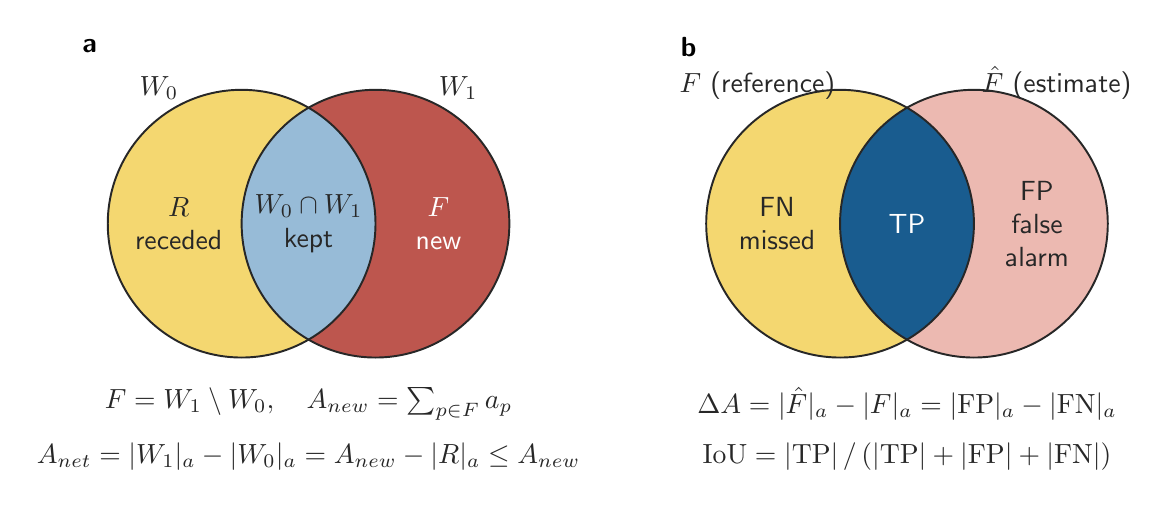
\begin{tikzpicture}[font=\normalsize, line width=0.7pt]
% ---------------- (a) water states
\node[font=\bfseries, anchor=west] at (-3.0,2.25) {a};
\def\Wzero{(-0.85,0) circle (1.7)}
\def\Wone{(0.85,0) circle (1.7)}
\fill[cR!70] \Wzero;
\fill[cF] \Wone;
\begin{scope}\clip \Wzero; \fill[cW0!55] \Wone; \end{scope}
\draw[cInk] \Wzero; \draw[cInk] \Wone;
\node[cInk, anchor=south] at (-1.9,1.45) {$W_0$};
\node[cInk, anchor=south] at (1.9,1.45) {$W_1$};
\node[align=center, cInk] at (-1.65,0) {$R$\\receded};
\node[align=center, cInk] at (0,0) {$W_0\cap W_1$\\kept};
\node[align=center, white] at (1.65,0) {$F$\\new};
\node[anchor=north, cInk] at (0,-1.95) {$F = W_1\setminus W_0,\quad A_{new}=\textstyle\sum_{p\in F} a_p$};
\node[anchor=north, cInk] at (0,-2.65) {$A_{net}=|W_1|_a-|W_0|_a = A_{new}-|R|_a \le A_{new}$};
% ---------------- (b) estimate vs reference
\begin{scope}[xshift=7.6cm]
\node[font=\bfseries, anchor=west] at (-3.0,2.25) {b};
\def\Fref{(-0.85,0) circle (1.7)}
\def\Fhat{(0.85,0) circle (1.7)}
\fill[cFN!70] \Fref;
\fill[cFP] \Fhat;
\begin{scope}\clip \Fref; \fill[cTP] \Fhat; \end{scope}
\draw[cInk] \Fref; \draw[cInk] \Fhat;
\node[cInk, anchor=south] at (-1.9,1.45) {$F$ (reference)};
\node[cInk, anchor=south] at (1.9,1.45) {$\hat F$ (estimate)};
\node[align=center, cInk] at (-1.65,0) {FN\\missed};
\node[align=center, white] at (0,0) {TP};
\node[align=center, cInk] at (1.65,0) {FP\\false\\alarm};
\node[anchor=north, cInk] at (0,-1.95) {$\Delta A=|\hat F|_a-|F|_a=|\mathrm{FP}|_a-|\mathrm{FN}|_a$};
\node[anchor=north, cInk] at (0,-2.65) {$\mathrm{IoU}=|\mathrm{TP}|\,/\,(|\mathrm{TP}|+|\mathrm{FP}|+|\mathrm{FN}|)$};
\end{scope}
\end{tikzpicture}
\end{document}
